\documentclass[10pt, titlepage]{article}

\usepackage[margin=1in]{geometry}
\usepackage{fancyhdr}
\usepackage{amsfonts}
\usepackage{amsmath}
\usepackage{amssymb}
\usepackage{booktabs}
%\usepackage{tikz}
\usepackage{nicematrix}
\usepackage{float}
\usepackage{bm}
\usepackage{pgfplots}


\title{\normalsize PLUS Session Worksheet \\[1em] \Large \textit{MATH 1554:} Linear Algebra}
\author{\textit{Covering Section:} 5.9}
\date{Fall 2023}

% ------- Set up header -------
\renewcommand{\sectionmark}[1]{\markright{#1}} % from https://tex.stackexchange.com/a/317393/227665
\pagestyle{fancy}
\fancyhead[L]{A. M., Fall 2023}
%\fancyhead[C]{\textit{\nouppercase{\rightmark}}}
\fancyhead[C]{\textit{Markov Chains (5.9)}}
\fancyhead[R]{\textbf{\thepage}}
% -------------------------------------------------------

% ------- Set up question environment -------
\newcounter{question}
\setcounter{question}{1}
\newenvironment{newquestion}
{
	\noindent\textbf{Question \thequestion}
}
{
\stepcounter{question}
\par
}
% -------------------------------------------------------

% ------- Set up Main Idea box environment -------
\newcounter{mainideas}
\setcounter{mainideas}{1}
\newcommand{\mainidea}{\textbf{Main Idea \#\themainideas \stepcounter{mainideas}}}
\setlength\fboxsep{1em}
%\newcommand{\midea}[2]{\begin{center}\fbox{\parbox{#1}{\centering \mainidea #2}} \end{center}} % Could be environment but I couldn't bother

% The way this works is that the savebox collects whatever was between the minipage and the end of it, then in the last line of the definition of the environment
% we regurgigate whatever was collected into an fbox which we center.
\newsavebox{\mybox}
\newenvironment{mideea}[1]
{%
\begin{lrbox}{\mybox}%
	\begin{minipage}{#1\textwidth}
		{\centering \mainidea \par}

}
{\end{minipage}\end{lrbox}\begin{center}\fbox{\usebox{\mybox}}\end{center}}
% -------------------------------------------------------


% ------- Set up math stuff -------
\renewcommand{\vec}[1]{\bm{#1}}
\DeclareMathOperator{\vspan}{Span}
\DeclareMathOperator{\row}{row}
\DeclareMathOperator{\col}{col}
\DeclareMathOperator{\colspace}{Col}
\DeclareMathOperator{\rowspace}{Row}
\DeclareMathOperator{\nullspace}{Nul}
\DeclareMathOperator{\rank}{rank}
\DeclareMathOperator{\proj}{proj}
% -------------------------------------------------------

% ------- Set up circle -------
\newcommand{\bubble}{\tikz[baseline=-0.625ex]\draw[radius=0.5em, fill=white] (0,0) circle;}
\newcommand{\dbubble}{\tikz[baseline=-0.625ex]\draw[radius=0.5em, fill=black] (0,0) circle;}
% -------------------------------------------------------

\makeatletter
\setlength{\@fptop}{0pt}
\makeatother

\begin{document}
\maketitle

\section*{\centering Markov Chains (5.9)}
\subsection{T/F Questions}
\begin{newquestion}
	For each statement, mark the statement \emph{true} if it's \emph{always} true, or \emph{false} otherwise.
	\begin{table}[!h]
		\centering
		\begin{tabular}{c@{\hspace{2.5em}}cp{0.75\textwidth}}
			true & false & \\
			\specialrule{\lightrulewidth}{0.25em}{1.25em}
			\bubble & \bubble & Every stochastic matrix has a steady state vector. \\[0.75em]
			\bubble & \bubble & Only regular stochastic matrices have a unique probability steady state vector.\\[0.75em]
			\bubble & \bubble & The set of probability vectors in \(\mathbb{R}^3\) forms a subspace.\\[0.75em]
			\bubble & \bubble & Given two probability vectors \(\vec{x}, \vec{y} \in \mathbb{R}^3\), the vector \(2/3\vec{x} + 1/3\vec{y}\) is a probability 
						      vector as well.\\[0.75em]
			\bubble & \bubble & If \(P\) is a \(n \times n\) stochastic matrix, and \(\vec{x}_0 \in \mathbb{R}^n\) is a probabilty vector, then
						      \(\vec{x}_{k} = P^k\vec{x}_0\) is the probabilty vector that denotes the likelyhood that we're in a specific
						      state after applying \(P\) for \(k\) number of times after we've started off from \(\vec{x}_0\).\\[0.75em]
			\bottomrule
		\end{tabular}
	\end{table}
\end{newquestion}

\subsection{Short Answer Questions}
\begin{newquestion}
	For each question, provide your work and answer.
	\begin{enumerate}
		\item Consider the below transition diagram. Find the corresponding stochastic matrix, and then find the long-term trend of the Markov chain.
	\begin{figure}[!h]
		\centering
		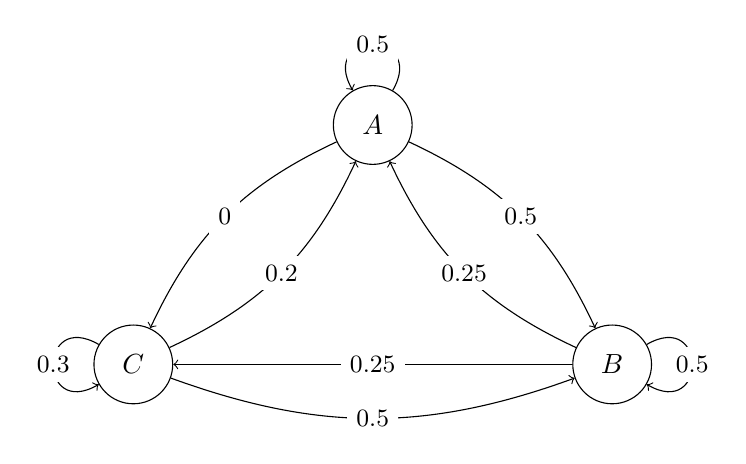
\begin{tikzpicture}[thin, node distance=43mm, main/.style = {draw, circle, minimum size=1cm}, lbl/.style={midway, fill=white, font=\small}]
			\node[main] (A) {\(A\)};
			\node[main] (B) [below right of=A] {\(B\)};
			\draw[bend left=20, ->] (A) to node[lbl] {0.5} (B);
			\draw[bend left=20, ->] (B) to node[lbl] {0.25} (A);

			\node[main] (C) [below left of= A] {\(C\)};
			\draw[bend right=20, ->] (A) to node[lbl] {0} (C);
			\draw[bend right=20, ->] (C) to node[lbl] {0.2} (A);

			\draw[->] (B) to node[lbl] {\small 0.25} (C);
			\draw[bend right=20, ->] (C) to node[lbl] {0.5} (B);

			\draw[->] (A) to [out=60, in=120, looseness=4.5] node[lbl] {0.5} (A);
			\draw[->] (B) to [out=30, in=330, looseness=4.5] node[lbl] {0.5} (B);
			\draw[->] (C) to [out=150, in=210, looseness=4.5] node[lbl]{0.3} (C);
		\end{tikzpicture}
	    \end{figure}

		\item Given what you know, what would you say is \(\det(P - I)\), for any stochastic matrix \(P\)?
	\end{enumerate}
\end{newquestion}

\section{\centering Solutions}

\subsection{Solutions to T/F Questions}
	\begin{table}[!h]
		\centering
		\begin{tabular}{c@{\hspace{2.5em}}cp{0.75\textwidth}}
			true & false & \\
			\specialrule{\lightrulewidth}{0.25em}{1.25em}
			\dbubble & \bubble & Every stochastic matrix has a steady state vector. \\[0.75em]
			\bubble & \dbubble & Only regular stochastic matrices have a unique probability steady state vector.\\[0.75em]
			\bubble & \dbubble & The set of probability vectors in \(\mathbb{R}^3\) forms a subspace.\\[0.75em]
			\dbubble & \bubble & Given two probability vectors \(\vec{x}, \vec{y} \in \mathbb{R}^3\), the vector \(2/3\vec{x} + 1/3\vec{y}\) is a probability 
						      vector as well.\\[0.75em]
			\dbubble & \bubble & If \(P\) is a \(n \times n\) stochastic matrix, and \(\vec{x}_0 \in \mathbb{R}^n\) is a probabilty vector, then
						      \(\vec{x}_{k} = P^k\vec{x}_0\) is the probabilty vector that denotes the likelyhood that we're in a specific
						      state after applying \(P\) for \(k\) number of times after we've started off from \(\vec{x}_0\).\\[0.75em]
			\bottomrule
		\end{tabular}
	\end{table}

\subsection{Solutions to Short Answer Questions}
	\begin{enumerate}
		\item There are actually multiple valid answers for this question. So, please note the states the columns correspond to.
			\NiceMatrixOptions{
				code-for-first-row=\color{teal},
				code-for-first-col=\color{purple},
			}
			\[
				\begin{bNiceMatrix}[first-row,first-col]
				   	&   A   &   B   &    C   \\
				     A & 0.5  & 0.25 & 0.2 \\
				     B & 0.5  &  0.5  & 0.5 \\
				     C &  0   &  0.25 & 0.3
				\end{bNiceMatrix}
			\]
			The states in teal denote the {\color{teal} from}, and the states in purple denote the states that {\color{purple} receive}.
		\item Finding the ``long-term trend" of the chain corresponds to finding the steady-state vector. 
			\begin{align*}
				\begin{bmatrix}0.5 & 0.25 & 0.2 \\ 0.5 & 0.5 & 0.5 \\ 0 & 0.25 & 0.3\end{bmatrix} - I_3 &= 
				\begin{bmatrix}-0.5 & 0.25 & 0.2 \\ 0.5 & -0.5 & 0.5 \\ 0 & 0.25 & -0.7\end{bmatrix} 
				\sim \begin{bmatrix}0.5 & -0.5 & 0.5 \\ 0 & -0.25 & 0.7 \\ 0 & 0.25 & -0.7\end{bmatrix} \\[0.5em]
				&\sim \begin{bmatrix}1 & -1 & 1 \\ 0 & 1 & - 14/5 \\ 0 & 0 & 0\end{bmatrix} 
				\sim \begin{bmatrix}1 & 0 & 1 - 14/5 \\ 0 & 1 & -14/5 \\ 0 & 0 & 0\end{bmatrix}
			\end{align*}
			From here we see that \(\vec{x} = t\begin{bmatrix}9/5 \\ 14/5 \\ 1\end{bmatrix}.\) However, the sum of the entries should add up to one, and
			so \(\vec{q} = \displaystyle \frac{5}{28}\begin{bmatrix}9/5 \\ 14/5 \\ 1\end{bmatrix}.\)
		
			You can verify that this is the steady-state vector by left-nultiplying it with the matrix.
		
		\item It's always 0.
	\end{enumerate}
\end{document}